%% This layout has been constructed from the combination of several packages, layout found on internet and from my own construction. 
%% It is done to match the layout of Centrale Méditerranée but can be adapted for other university
%% Author: Vincent G. 2025 (Promo Entrante 2022)


\documentclass[11pt]{memoir}

% Front page (Replace with your own information)
\newcommand{\prenomNOM}{ZHAO Chao} % prénom NOM
\newcommand{\dateDebutStage}{01/04/2025} % jour/mois/année
\newcommand{\dateFinStage}{01/10/2025} % jour/mois/année
\newcommand{\nomEntreprise}{École nationale des ponts et chaussées} % Nom de l'entreprise 
\newcommand{\sujetMission}{DigiEV: A digital twin for electric vehicle charging
infrastructure in the E4C ecosystem} % Sujet de mission 
\newcommand{\supervisor}{Dr.Daphne Tuncer (École des ponts)}
\newcommand{\cosupervisor}{Dr.Georgios Bouloukakis (Télécom SudParis)}
\newcommand{\attestation}{
  \vskip 0.5em
  \justifying
  Je, soussignée Daphne Tuncer, maître de stage de l'élève Isep, ZHAO Chao, atteste avoir pris connaissance du
  cahier des charges du rapport de stage Isep, avoir lu et évalué le présent rapport au regard
  du cahier des charges et des pratiques de mon employeur, et autorisée sa transmission à l'Isep.
  \vskip 0.5em
  \hfill Signature / Date :
}





\setlength{\headheight}{14.80524pt}
%%% Packages %%%
\usepackage{multirow}
\usepackage[T1]{fontenc}
\usepackage{ragged2e}
\usepackage{listings}
%%\usepackage[latin1, utf8]{inputenc}
\usepackage{lmodern} 
\usepackage[a4paper,right=2.75cm, left=2.75cm, top=3.cm, bottom=4.cm]{geometry}
\usepackage[english]{babel} % You can change to english if needed
\usepackage{afterpage}
\usepackage[colorlinks=true, urlcolor=blue, citecolor=blue, linkcolor=black]{hyperref}
% \setSingleSpace{1.1} % Space between lines of the text
\usepackage{calc, blindtext}
\usepackage[table]{xcolor}
\usepackage{nicematrix, booktabs}
\usepackage{graphicx,soul}
\usepackage{enumitem,lipsum}
\usepackage{float} % For the [H] option in tables
\usepackage{minted}
\usepackage{adjustbox}
\usepackage{mathtools,amsfonts,amsthm,amssymb,amsmath}
\usepackage{fancyvrb}  % pour afficher proprement du code LaTeX
\usepackage{array}
\usepackage{siunitx}
\sisetup{detect-all} % note: just one option still needs to be specified
\usepackage{tikz}
\definecolor{doc}{RGB}{0,60,110}
\usepackage{titletoc}
\setcounter{tocdepth}{3}
\usepackage{pdfpages}
\usepackage{titletoc}
\usepackage[figurename=Fig., tablename=Tab.]{caption}
\usepackage{subcaption}
\usepackage[acronym]{glossaries}
\makeglossaries
\usepackage{nameref}
\renewcommand{\thesection}{\arabic{section}}

%%% Colors %%%
\definecolor{CentraleBlue}{RGB}{11,15,157}   % Blue of the Centrale Med Logo
\definecolor{codebg}{rgb}{0.95,0.95,1}       % Light blue background for the code box

%%% Custom Chapter Style %%%
\makechapterstyle{HansenColor}{
  \chapterstyle{Hansen}               
  \renewcommand{\printchaptername}{}  % Remove "Chapter" word
  \renewcommand{\printchapternum}{}   % Remove chapter number
  \renewcommand{\afterchapternum}{}   % Remove spacing left by the number

  % Set the chapter title in blue (customize color as needed)
  \renewcommand*{\printchaptertitle}[1]{\chaptitlefont\color{CentraleBlue}##1} 
}

%%% Maths %%% 

% Theorems, definitions, propositions etc.
\theoremstyle{plain}
\newtheorem{theorem}{Théorème}[section]
\newtheorem{proposition}[theorem]{Proposition}
\newtheorem{lemma}[theorem]{Lemme}
\newtheorem{corollary}[theorem]{Corollaire}

\theoremstyle{definition}
\newtheorem{definition}[theorem]{Définition}
\newtheorem{remark}[theorem]{Remarque}

% You can define your own commands
\newcommand{\R}{\mathbf{R}}
\newcommand{\N}{\mathbf{N}}
\newcommand{\Q}{\mathbf{Q}}
\newcommand{\Z}{\mathbf{Z}}
\newcommand{\CC}{\mathbf{C}}
\newcommand{\E}{\mathbf{E}}
\newcommand{\D}{\ensuremath{\mathrm{d}}}
\newcommand{\Cov}{\mathrm{Cov}}
\newcommand{\Var}{\mathrm{Var}}

\usepackage{fancyhdr}
\pagestyle{fancy}
\renewcommand\chaptermark[1]{\markboth{\thechapter: \enskip#1}{}}
\renewcommand\sectionmark[1]{\markright{\thesection:\enskip#1}{}}
\fancyhf{}

\fancyhead[LE]{%
  \makebox[0pt][r]{
    \colorbox{CentraleBlue}{\makebox[\textwidth][r]{\bfseries\textcolor{white}{\thepage}\enskip}}\hspace*{1em}}{\itshape\rightmark}\hspace*{1em}\headrulefill%
}

\fancyhead[RO]{%
  \mbox{}\headrulefill \hspace*{1em}{\itshape\leftmark}%
  \makebox[0pt][l]{%
    \hspace*{1em}\colorbox{CentraleBlue}{\makebox[\textwidth][l]{\enskip\bfseries\textcolor{white}{\thepage}}}}%
}
\renewcommand\headrulewidth{0pt}

\def\headrulefill{\leaders\hrule width 0pt height 3pt depth -2.8pt \hfill}

% Redefine the plain page style
\fancypagestyle{plain}{
    \fancyhead[LE]{%
    \makebox[0pt][r]{
    \colorbox{CentraleBlue}{\makebox[\textwidth][r]{\bfseries\textcolor{white}{\thepage}\enskip}}\hspace*{1em}}%
      {\itshape\leftmark}\hspace*{1em}\headrulefill%
    }
    \fancyhead[RO]{%
    \mbox{}\headrulefill \hspace*{1em}{\itshape\leftmark}%
    \makebox[0pt][l]{%
    \hspace*{1em}\colorbox{CentraleBlue}{\makebox[\textwidth][l]{\enskip\bfseries\textcolor{white}{\thepage}}}}%
    }
    \renewcommand\headrulewidth{0pt}

     \setlength{\headheight}{14.32591pt}
     
    \def\headrulefill{\leaders\hrule width 0pt height 3pt depth -2.8pt \hfill}
}

% Caption style
\DeclareCaptionFormat*{custom}{
    \renewcommand{\arraystretch}{0.05}
    \centering
    \hspace{-25pt} 
    \begin{tabular}{p{45pt}@{\hspace{0.0em}} !{\color{CentraleBlue}\vrule width 2pt} p{0.9\linewidth-30pt}}
    \hspace{-0.05\linewidth} {\colorbox{CentraleBlue}{\parbox[t][10pt][l]{38pt}{\bfseries\textcolor{white}{#1}}}}
    & \parbox[t]{\linewidth}{#3}
    \end{tabular}
}

\captionsetup{format=custom, labelsep=none, indention=0pt} % comment if you don't want to use the red boxes


\makeatletter
\newlength\dlf@normtxtw
\setlength\dlf@normtxtw{\textwidth}
%\def\myhelvetfont{\def\sfdefault{mdput}}
\newsavebox{\feline@chapter}
\newcommand\feline@chapter@marker[1][4cm]{
    \sbox\feline@chapter{%
    \resizebox{!}{#1}{\fboxsep=1pt%
      \colorbox{CentraleBlue}{\parbox[t][3mm][c]{2.5mm}{\centering\color{white}\bfseries\sffamily\thechapter}}%
    }}%
  \rotatebox{90}{%
    \resizebox{%
      \heightof{\usebox{\feline@chapter}}+\depthof{\usebox{\feline@chapter}}}%
    {!}{\scshape\so\@chapapp}}\quad%
  \raisebox{\depthof{\usebox{\feline@chapter}}}{\usebox{\feline@chapter}}%
}
\newcommand\feline@chm[1][4cm]{%
  \sbox\feline@chapter{\feline@chapter@marker[#1]}%
  \makebox[0pt][l]{% aka \rlap
    \makebox[1cm][r]{\usebox\feline@chapter}%
  }}
  
\makechapterstyle{daleif1}{
  \renewcommand\chapnamefont{\normalfont\Large\scshape\raggedleft\so}
  \renewcommand\chaptitlefont{\normalfont\huge\bfseries\scshape\color{CentraleBlue}}
  \renewcommand\chapternamenum{}
  \renewcommand\printchaptername{}
  \renewcommand\printchapternum{\null\hspace{\textwidth-1cm}\feline@chm[0.35cm]\par}
  \renewcommand\afterchapternum{\par\vskip\midchapskip}
  \renewcommand\printchaptertitle[1]{\chaptitlefont\raggedleft ##1\par}
}

\setlist[itemize]{itemsep=\parskip, parsep=0pt}
\setlist[enumerate]{itemsep=\parskip, parsep=0pt}

\makeatother


\chapterstyle{HansenColor}

\begin{document}

\setcounter{secnumdepth}{3}
\thispagestyle{empty}
\newcommand{\HRule}{\rule{\linewidth}{0.5mm}} % épaisseur de lignes horizontales
\setlength\fboxrule{2pt} % épaisseur de la boîte de mission
\newgeometry{top=2cm, bottom=1cm, left=2cm, right=2cm}

%----------------------------------------------------------------------------------------
%	SECTION LOGO
%----------------------------------------------------------------------------------------
\begin{center}
    \adjustbox{valign=c}{
\includegraphics[width=3cm]{Images/isep.png}}
    \hspace{1.5cm}
    \adjustbox{valign=c}{
\includegraphics[width=6cm]{Images/logo-enpc-ip-rvb.jpg}}
    \hspace{1cm}
    \adjustbox{valign=c}{
\includegraphics[width=5cm]{Images/logo_tsp.png}}
\end{center}

%--------------------------prenomNOM--------------------------------------------------------------
%	SECTION TITRE
%----------------------------------------------------------------------------------------
\begin{center}
\definecolor{lightgray}{gray}{0.9}
\vskip 3em
\fcolorbox{black}{lightgray}{
    \begin{minipage}[c][5em][c]{0.9\textwidth}
        \centering
        \textbf{\LARGE\sujetMission}
    \end{minipage}
}
\vskip 3em
\Large\textbf{\LARGE Report of End of Studies Internship (IS.3001)}
\vskip 0.5em
presented by \textbf{\prenomNOM}
\vskip 0.5em
student id: \textbf{63315}

\end{center}

% %----------------------------------------------------------------------------------------
% %	SECTION MISSION DE STAGE
% %----------------------------------------------------------------------------------------
% \begin{center}
%     \Large
%     \definecolor{lightgray}{gray}{0.9}
%     \vskip 2em
%     \fcolorbox{black}{lightgray}{
%         \begin{minipage}[c][6em][c]{0.9\textwidth}
%             \centering
%             \textbf{\sujetMission}
%         \end{minipage}
%     }
%     \end{center}


%----------------------------------------------------------------------------------------
% SECTION TUTEUR/DIRECTEUR STAGE
%----------------------------------------------------------------------------------------
\begin{center}
\Large
\vskip 3em
Internship from \dateDebutStage \ to \dateFinStage \ at :
\vskip 0.5em
\textbf{\nomEntreprise}
\vskip 2em
\begin{minipage}[l]{0.95\textwidth}
    \begin{flushleft}
    Supervisor : \textbf{\supervisor}
    \vskip 0.5em
    Co-Supervisor : \textbf{\cosupervisor}
    \end{flushleft}
    \vskip 1em
    \HRule
\end{minipage}
\end{center}
%----------------------------------------------------------------------------------------
% SECTION BAS DE PAGE
%----------------------------------------------------------------------------------------
\begin{center}
\Large
\vskip 1em
Attestation du maître de stage : \attestation
\end{center}
\vfill % remplit le reste de la page avec des espace

\restoregeometry
\cleardoublepage
\normalsize


\newgeometry{top=3cm, bottom=1cm, left=2cm, right=6cm}  % set new margins


% --- Remerciements ---
\chapter*{Acknowledgments}

I would like to sincerely thank my supervision team, Dr.Daphne Tuncer and Dr.Georgios Bouloukakis, for their continuous guidance, insightful advice, and encouragement throughout this six-month internship. Their expertise not only supported my R\&D tasks but also inspired me to explore the world of academic research, opening a new path in my professional journey.

I am also deeply grateful to my wife, WANG Yaoyao, for her unconditional support in daily life. Her encouragement has been a vital source of strength during this period. In addition, I would like to express my heartfelt gratitude to my parents, whose love, trust, and support have always been the foundation of my personal and professional growth. All their constant encouragement has given me the confidence to pursue new challenges and persist through difficulties.

Lastly, I would like to acknowledge E4C for providing the resources and support that made this internship possible.


% \bigskip
% % \begin{center}
% %     \Huge * * *
% % \end{center}

\newpage


% --- Abstract ---

\chapter*{Abstract}
% ENGLISH ABSTRACT

The success of electric mobility requires not only advanced electric vehicles but also an integrated infrastructure that combines electricity provision, information distribution, and intelligent system control. Digital twin technology has emerged as a powerful approach to manage complex infrastructure operations and evaluate deployment strategies for electric vehicle charging networks~\cite{Yu2024}.

This report describes the work conducted during my six-month internship at Laboratoire Ville Mobilité Transport (LVMT) - École nationale des ponts et chaussées (ENPC), focusing on the design and development of a digital twin system to simulate the energy impact of electric vehicle charging infrastructure. The project employed FIWARE technology as the core framework, utilizing Python for system development and data processing to model the complex interactions between energy consumption and user behavior in charging station.

The developed digital twin system successfully established a comprehensive platform for simulating charging station operations, built upon NGSI-LD standard compliance to ensure semantic interoperability. The system utilizes MongoDB and CrateDB as backend databases for efficient data storage and time-series analysis, while providing RESTful API interfaces for seamless system integration and external interactions. This platform enables real-time monitoring and analysis of charging infrastructure performance, providing valuable insights for optimizing charging station deployment, predicting energy demand patterns, and improving overall system efficiency. The work contributes to enhanced decision-making capabilities for electric vehicle charging infrastructure planning and management through standardized data models and accessible programming interfaces.

This internship significantly enhanced my technical expertise. Additionally, I strengthened my research skills through extensive literature review and analysis of current challenges in sustainable transportation infrastructure. The experience provided valuable insights into the interdisciplinary nature of smart city technologies and the critical role of digital twins in managing complex urban systems.

\bigskip\bigskip

\textbf{\color{CentraleBlue}Keywords} Digital Twin, Simulator, Semantic Model, Electric Vehicle, Charging Infrastructure, FIWARE

\newpage

\restoregeometry 

\tableofcontents

%%% Chapters %%%
\chapter{Introduction}\label{chap1}

The global transition toward electric mobility is regarded as a cornerstone of 
efforts to decarbonize the transport sector and meet international climate 
targets. According to the International Energy Agency, electric car sales 
reached nearly 14 million in 2023, and are projected to exceed 17 million 
in 2024, representing more than one-fifth of global car sales~\cite{IEA2024}. 
However, this rapid diffusion of electric vehicles (EVs) poses systemic 
challenges that extend beyond vehicle manufacturing. The widespread adoption 
of EVs crucially depends on the development of robust charging infrastructure 
and the integration of energy systems capable of supporting increasing loads 
while ensuring reliability and user acceptance~\cite{Metais2022}. 

Charging infrastructure represents both a key enabler and a potential bottleneck 
in the electrification of mobility. Without adequate charging coverage, 
prospective EV users may face range anxiety, undermining confidence in the 
technology and slowing adoption~\cite{Metais2022}. At the same time, 
deploying charging networks entails high capital costs and introduces 
technical challenges related to grid integration, station placement, and 
operational optimization. France, for instance, has set ambitious goals of 
400,000 publicly accessible charging points by 2030, yet as of 2023 fewer 
than 100,000 had been deployed, revealing the scale of investment and 
coordination required~\cite{Autorite2023}. This "chicken-and-egg"
problem—insufficient infrastructure limiting EV adoption, while weak demand 
discourages infrastructure investment—highlights the importance of 
strategically planned deployment~\cite{Bernard2021}.

To address these challenges, advanced modeling and simulation tools have been 
proposed to guide infrastructure planning and management. Digital twin 
technology, in particular, offers a powerful approach to replicate complex 
physical systems in a virtual environment, enabling real-time monitoring, 
scenario evaluation, and predictive analytics. Recent studies highlight the 
potential of digital twins to support the integration of charging infrastructure 
with smart grids, optimize location and capacity decisions, and enhance 
decision-making under uncertainty~\cite{Charette2023, Metais2022}. 


This report builds upon this context by presenting the work conducted during 
a six-month internship at the Laboratoire Ville Mobilité Transport (LVMT), 
École nationale des ponts et chaussées (ENPC). The project focused on the 
design and development of a digital twin system for simulating the energy 
impact of EV charging infrastructure, employing the FIWARE framework and 
NGSI-LD standards to ensure interoperability. By coupling backend databases 
(MongoDB, CrateDB) with real-time APIs, the system provides a scalable 
platform for monitoring charging operations and assessing deployment 
strategies. The work contributes to ongoing research in sustainable mobility 
by demonstrating how digital twins can support the optimization of EV 
charging infrastructure within smart city ecosystems.

This report is organized into seven main chapters, each addressing specific aspects 
of the internship work and its broader context:

Chapter 2~\textbf{\nameref{chap2}} first introduces the institutional framework, including ENPC, LVMT and E4C. It then describes the supervision and project framework. Finally, it outlines the research background, covering energy and environmental challenges in transport, electric vehicles and charging infrastructure, digital twin and simulation, as well as data models and interoperability.

Chapter 3~\textbf{\nameref{chap3}} examines existing technologies, 
including FIWARE, BRICK, Web of Things (WoT). This chapter also identifies current challenges and positions our contribution within the 
existing body of knowledge.

Chapter 4~\textbf{\nameref{chap4}} details the system architecture, semantic data modeling 
approach using NGSI-LD, backend database implementation, API subscription mechanism, and 
visualization components. It concludes with an analysis of difficulties 
encountered, and deviations from initial specifications.

Chapter 5~\textbf{\nameref{chap5}} presents the definition and 
initialization of three experimental scenarios, results obtained using both real 
and synthetic data, and validation of the digital twin system performance.

Chapter 6~\textbf{\nameref{chap6}} addresses social and environmental 
responsibility aspects of the project and discusses innovation management and digital 
tools for decision-making in research.

Chapter 7~\textbf{\nameref{chap7}} summarizes the main outcomes of the internship and reflects the future work.At the same time, this chapter connects the technical achievements with personal growth and career prospects.  



\chapter{Context}\label{chap2}

\section{Institutional Framework}
This six-month internship was conducted at the \textbf{Laboratoire Ville Mobilité Transport (LVMT)}, a research unit affiliated with \textbf{École nationale des ponts et chaussées (ENPC)}, with funding provided by the \textbf{Energy4Climate interdisciplinary center (E4C)}. This institutional arrangement reflects the collaborative nature of contemporary energy and mobility research to address complex challenges in sustainable transportation infrastructure. The following sections detail the structure, missions, and research orientations of these three interconnected organizations that provided the framework for this research project.

\textbf{ENPC} represents one of France's most prestigious engineering institutions. Founded in 1747 by Daniel-Charles Trudaine, ENPC is among the oldest French Grandes Écoles, historically focused on training engineering officials and civil engineers. The school has evolved to offer wide-ranging education including computer science, applied mathematics, civil engineering, mechanics, finance, economics, innovation, urban studies, environment and transport engineering. In July 2024, ENPC became the sixth member school of Institut Polytechnique de Paris (IP Paris), joining École polytechnique, ENSTA Paris, ENSAE Paris, Télécom Paris and Télécom SudParis.

Located on the Champs-sur-Marne campus, ENPC maintains a strong international presence with 43\% of its students obtaining double degrees abroad and 30\% of the engineering cohort being international students. The institution's research excellence is supported by 12 research laboratories, covering domains crucial to ecological, digital, and energy transitions, positioning it as a key player in addressing contemporary sustainability challenges.

\textbf{LVMT} serves as the direct host institution for this research project. Created in 2003, this multidisciplinary research laboratory operates as a joint research unit between Université Gustave Eiffel and École nationale des ponts et chaussées. Celebrating its 20th anniversary in 2023, LVMT brings together nearly 90 researchers in social sciences and engineering sciences, with expertise spanning economics, anthropology, sociology, geography, urban planning, technical economics, mathematical modeling, and computer science.

The laboratory's scientific objective centers on understanding and modeling interactions between mobility practices, transport infrastructure, and spatial organization and development. Research activities are organized around four thematic axes: mobility practices and urban access; territorial dynamics and public action; city-transport interactions; and economic analysis and transport modeling. LVMT researchers collaborate extensively with national and international laboratories as well as public and private transport and urban planning stakeholders, including territorial authorities, public decision-makers, ADEME, RATP, SNCF, and Transdev. This collaborative approach combines quantitative methods and qualitative analyses, positioning the laboratory at the interface between academic research and action research.

\textbf{E4C} provides the funding framework and broader research context for this internship. Launched in June 2019 by IP Paris and ENPC, E4C addresses energy transition through research, training, and innovation. The center gathers 21 laboratories from Institut Polytechnique de Paris and 5 associated laboratories from ENPC, creating a unique interdisciplinary platform for energy and climate research.

Nearly 30 laboratories work within E4C on four cross-cutting themes designed to reduce greenhouse gas emissions, improve energy efficiency, deploy renewable energy, and propose relevant energy policies. The center combines diverse scientific disciplines including social and economic sciences, materials sciences and engineering, applied mathematics, computer science, and geophysics. E4C develops instrumental platforms, models for energy forecasting and prediction, and maintains a comprehensive data center: the E4C DataHub.

The framework of this internship within E4C directly aligns with the center's mission to foster interdisciplinary collaboration addressing energy transition challenges. The digital twin development for EV charging infrastructure contributes specifically to E4C's objectives of improving energy efficiency and supporting the deployment of sustainable transportation solutions, demonstrating the practical application of interdisciplinary research in addressing real-world sustainability challenges.

\section{Research Supervision and Project Framework}

\subsection{Research Supervision Team}

This internship project was conducted under the joint supervision of two tutors, 
reflecting the interdisciplinary nature of digital twin technologies and their 
application to energy mobility systems.

\textbf{Dr. Daphné Tuncer} is my supervisor from ENPC, specializing in 
digitalisation in the energy and mobility sectors.  Prior to joining ENPC, She spent many years in the UK Higher Education. Her research keywords include electric mobility, cyberphysical systems, data management, and applied data science.

\textbf{Dr. Georgios Bouloukakis} from Télécom SudParis, provides co-supervision with expertise in IoT/Edge-driven middleware and distributed software 
systems. He is an experienced researcher and educator with over one decade of teaching and mentoring of students, having supervised 2 postdoctoral researchers, 4 Ph.D. thesis, 4 R\&D developers and 48 bachelor/master theses. 

\subsection{Research Project Integration and Continuity}

This internship project represents a strategic extension of ongoing research within 
the E4C framework, building upon foundational work completed by previous interns 
while expanding into new application domains. The project directly follows the work 
of \textbf{Niemat Khoder}, who conducted her internship focusing on smart building energy 
management systems.

Niemat's research established important precedents for this work by demonstrating 
the application of NGSI-LD data models and semantic technologies in the building 
energy domain. Her thesis introduced a collaborative approach to optimizing energy 
management and enhancing occupant comfort through cross-building collaboration, 
leveraging NGSI-LD data models and developing the CCDUIT software tool for 
cross-federation collaboration. She successfully established "a modular, scalable, 
and interoperable framework for building data exchange" that enabled "enhanced 
energy efficiency through dynamic, real-time collaboration across energy management 
platforms."

The current project extends these foundational concepts from the building domain 
to electric vehicle charging infrastructure, maintaining the core principles of 
semantic interoperability and collaborative optimization while addressing the 
distinct challenges of mobility energy systems. Where Niemat's work focused on 
static building environments with predictable occupancy patterns, this project 
tackles the dynamic, spatially distributed nature of EV charging networks with 
highly variable user behavior and energy demand patterns.

Several key technical continuities link the two projects. Both leverage NGSI-LD 
as the semantic data modeling standard, ensuring consistency in data representation 
and interoperability approaches within the E4C research ecosystem. Both projects 
employ FIWARE as the core IoT platform, building institutional knowledge and 
technical expertise in this technology stack. The modular, scalable framework 
architecture pioneered in the building domain provides design principles that 
informed the charging infrastructure platform development.

However, the transition from buildings to mobility infrastructure required 
substantial methodological adaptations. The charging infrastructure domain demands 
real-time processing of energy consumption data across geographically distributed 
networks, necessitating the integration of time-series databases (CrateDB) alongside 
traditional document storage (MongoDB). The mobility context also requires more 
sophisticated simulation capabilities to model user behavior patterns and energy 
demand forecasting, leading to the development of comprehensive API interfaces 
for external system integration.

This project continuity reflects E4C's strategic approach to building cumulative 
research capabilities across related energy domains. By maintaining technical 
consistency while expanding application scope, the research program develops 
transferable methodologies and reusable technical components that can support 
future projects in sustainable energy system management.

The collaborative supervision model ensures both domain expertise in energy mobility 
(Dr. Tuncer) and technical depth in distributed IoT systems (Dr. Bouloukakis), 
providing the interdisciplinary foundation necessary to advance from building-focused 
research to the more complex challenges of transportation infrastructure digitalization.

\section{Research Background}

\subsection{Energy and Environment Challenges in Transport}

Transport is a central contributor to both energy use and environmental pressures. In France, it represented about 32\% of final energy consumption in 2023~\cite{IEA2025_FranceEnergy}, and around 66\% of total final consumption of oil products is attributable to transport~\cite{IEA2025_FranceOil}. It is also the largest national source of greenhouse-gas (GHG) emissions, accounting for approximately 32\% of territorial emissions in 2022, with road transport—cars and heavy vehicles—being the dominant contributors~\cite{HCC2023_GHG}.Beyond climate impacts, transport significantly contributes to local air pollution. The European Environment Agency notes persistent exposure to NO\textsubscript{2}, PM\textsubscript{2.5}, and ozone in urban areas with substantial health impacts~\cite{EEA2024_AirPollution}. 

Meeting these challenges requires a rapid shift toward low-carbon energy in transport. Electricity demand in France is projected to rise to 580-640 TWh by 2035, driven partly by electromobility; according to RTE, this scenario is feasible only with accelerated renewable deployment and smart charging strategies~\cite{RTE2023_Demand2035}. Therefore, electrifying mobility must be accompanied by a decarbonized electricity supply and effective demand-side management to deliver benefits for climate, air quality, and energy security.



\subsection{Electric Vehicles and Charging Infrastructure}

The rapid growth of electric vehicles (EVs) is transforming the transport and 
energy sectors. Global EV sales neared 14 million in 2023, accounting for 18\% of 
all new cars, with projections of around 17 million in 2024, or more than one-fifth 
of global car sales~\cite{IEA2024}. Yet the acceleration of EV adoption depends 
critically on the availability of suitable charging infrastructure.

EV charging infrastructure (EVCI) is both an enabler and a potential bottleneck of EV 
transition. Research highlights a persistent ``chicken-and-egg'' problem: users 
hesitate to purchase EVs without adequate charging coverage, while investors 
are reluctant to finance charging stations without a critical mass of EV users. 
Studies show that strategic deployment of charging points is more cost-effective 
than merely enlarging battery capacity, as infrastructure provision directly reduces 
range anxiety and supports large-scale diffusion~\cite{Metais2022}. 

From a planning perspective, charging infrastructure must address three 
dimensions: \emph{technical}, \emph{economic}, and \emph{user acceptance}. Technical 
issues involve compatibility of charging standards, grid integration, and power 
demand management. Economically, the high costs of fast-charging stations 
require careful location and sizing strategies. User acceptance hinges on 
convenience, accessibility, and charging time, which significantly influence EV 
adoption~\cite{LaMonaca2022}. 

\begin{figure}[ht!]
    \centering
    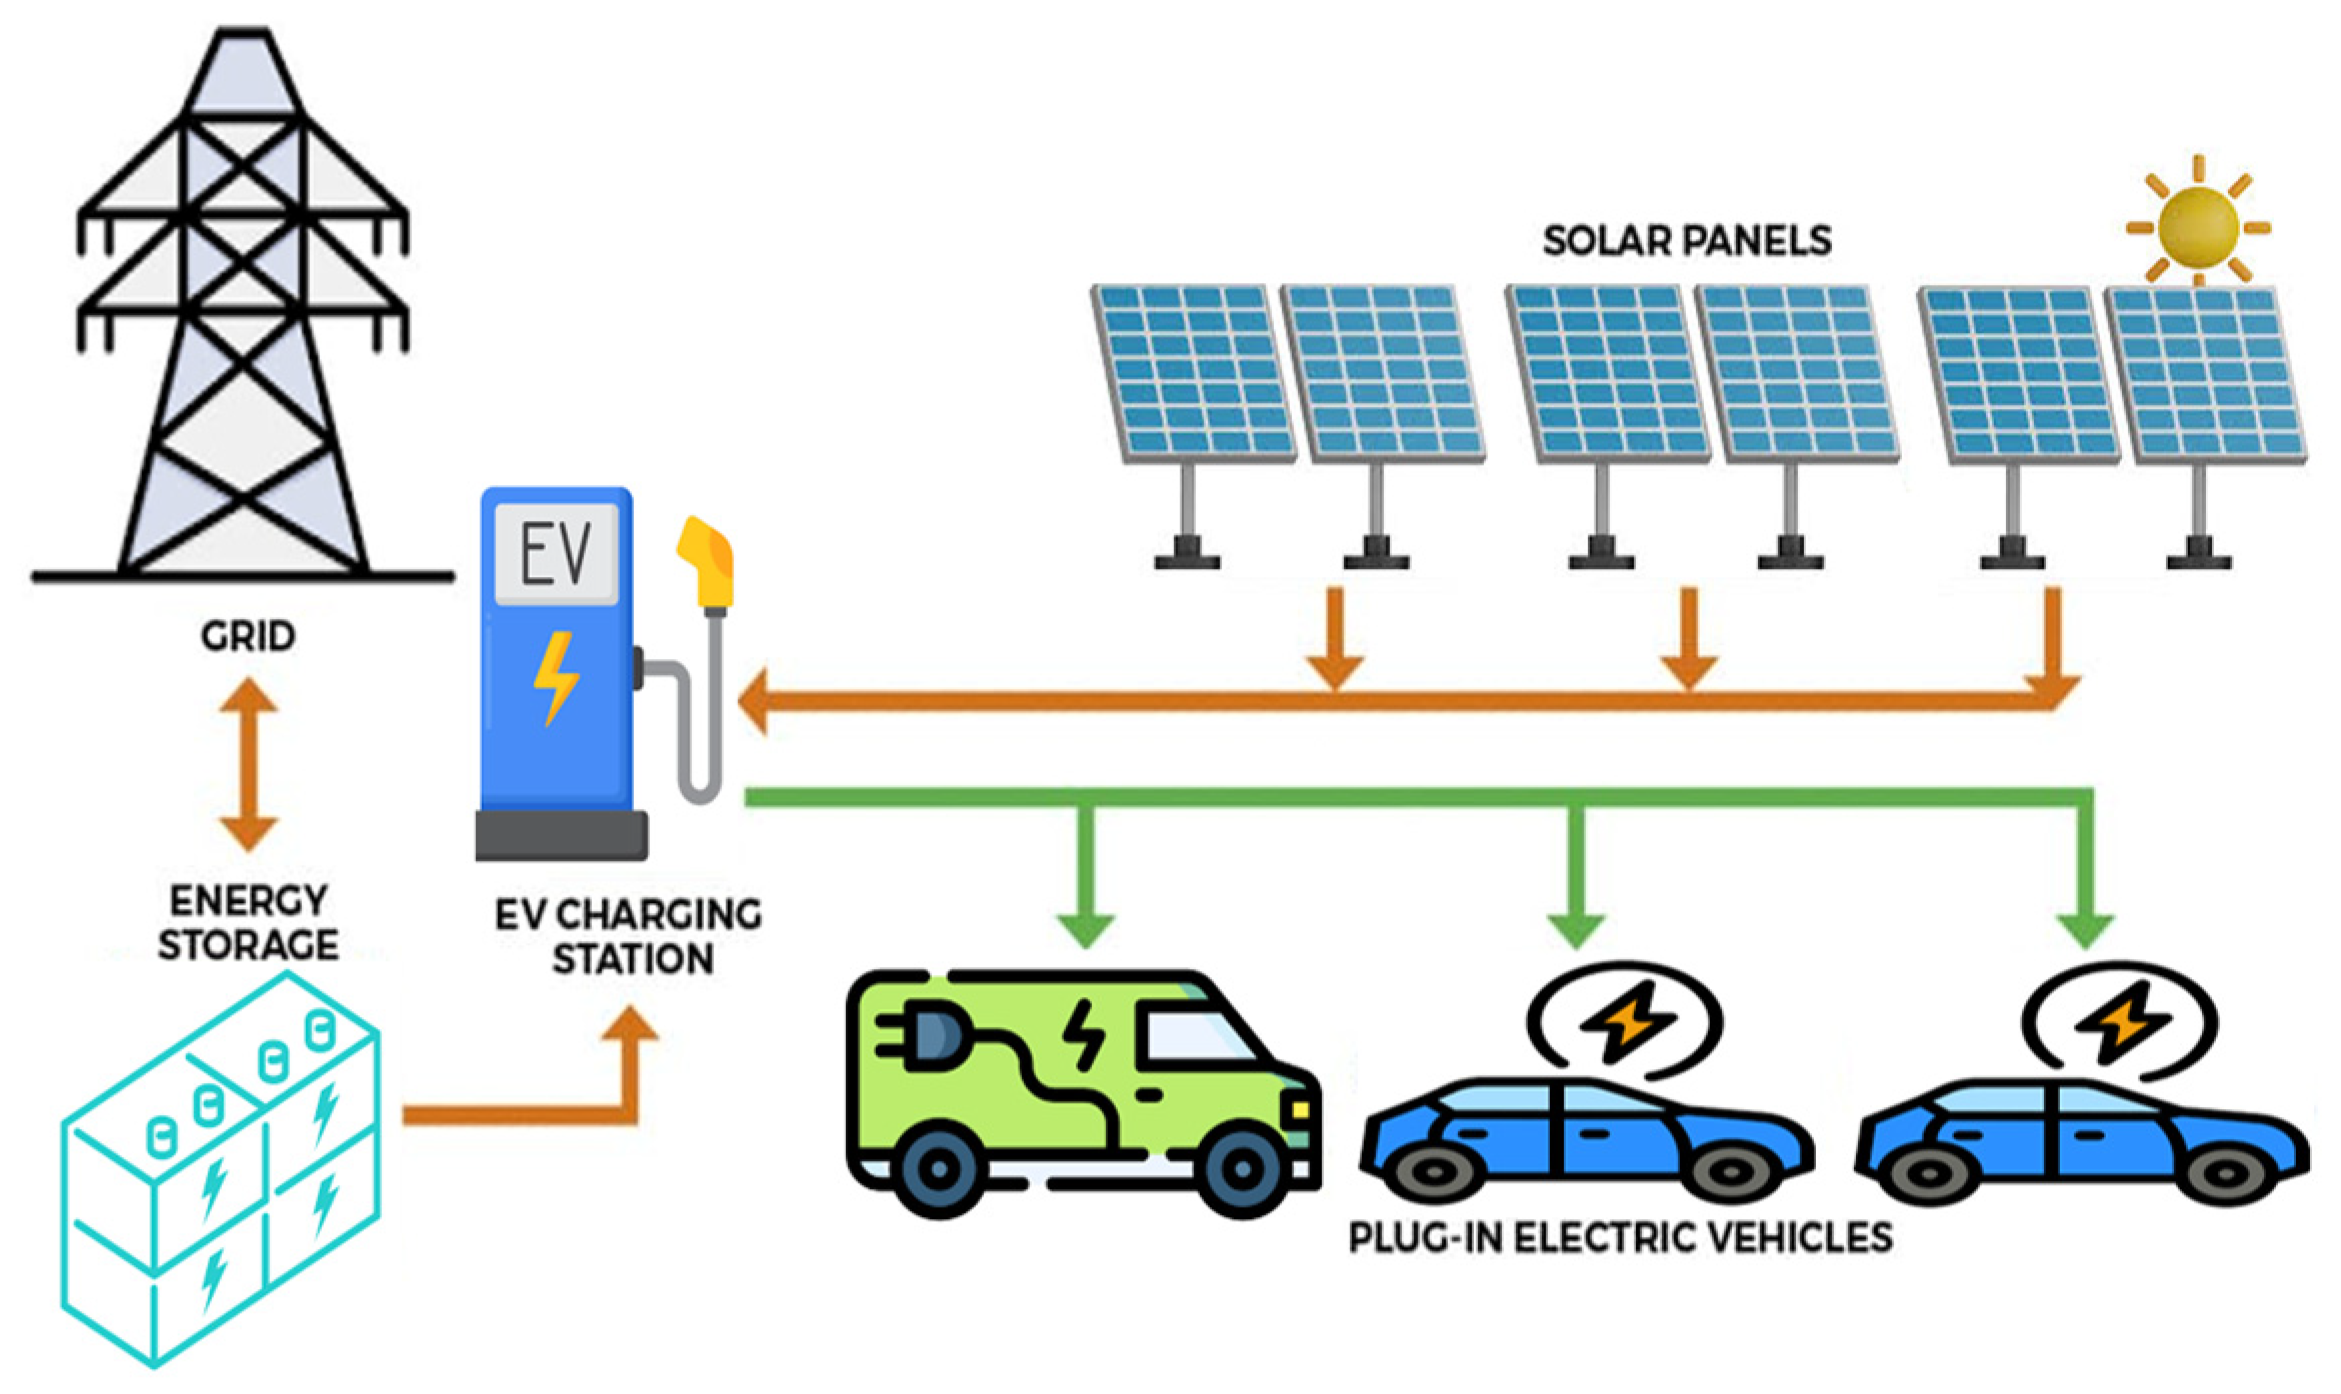
\includegraphics[width=0.7\textwidth]{Images/EVCI_diagram.png}
    \caption{\textbf{A typical EV charging infrastructure}~\cite{Deeum2023} \\Including electricity grid, 
    renewable generation (solar panels), energy storage systems, charging stations, 
    and plug-in electric vehicles. This integrated system highlights the importance of 
    coordinating generation, storage, and charging to ensure reliable and sustainable 
    operation.}
    \label{fig:EVCI_diagram}
\end{figure}

Emerging solutions aim to overcome these challenges. Dynamic charging, for 
instance, enables wireless on-road power transfer and has shown potential to 
reduce detours and charging time compared to conventional stations, though 
infrastructure costs remain high~\cite{Nguyen2024}. At the same time, digital twin 
technology is increasingly viewed as a powerful tool to manage the complexity 
of charging networks, enabling real-time monitoring, scenario analysis, and 
integration with renewable power and storage systems~\cite{Yu2024}. Such 
innovations highlight the importance of linking physical deployment with digital 
management systems to ensure reliability, sustainability, and scalability.

In summary, while EV adoption continues to expand rapidly, the success of the 
transition is inseparable from charging infrastructure. Planning, optimization, and 
digitalisation of charging networks will determine whether electrified transport 
can scale sustainably and equitably.

\subsection{Digital Twin and Simulation}

The increasing complexity of electric vehicle (EV) charging networks, 
their tight coupling with the power grid, and the variability of user 
behaviour make planning and operation challenging. Digital twin 
technology has emerged as a powerful approach to address these 
issues. A digital twin is defined as a ``live digital coupling of the state 
of a physical asset or process with a virtual representation that 
produces functional output''~\cite{Somers2023}. Unlike conventional 
models or static simulations, digital twins establish a continuous 
bi-directional link between the physical system and its digital replica, 
enabling real-time monitoring, predictive analytics, and feedback 
control~\cite{Liu2021Review,Enders2019}.

In the context of EV charging infrastructure, digital twins offer 
several advantages. First, they enable multi-scale simulation of 
charging demand and grid interaction, supporting optimal siting and 
sizing of charging stations. Second, they allow scenario analysis under 
uncertainty, including stochastic EV arrivals and variable renewable 
generation, thereby enhancing grid stability and resilience~\cite{Talusan2024}. 
Third, digital twins provide a platform for testing cyber-physical 
interactions, including cybersecurity assessment, without disrupting 
operational systems~\cite{Eckhart2019}. These capabilities make digital 
twin frameworks particularly suitable for managing charging networks 
within smart cities and integrating them into future vehicle-to-grid (V2G) 
and vehicle-to-building (V2B) systems.

\begin{figure}[ht!]
    \centering
    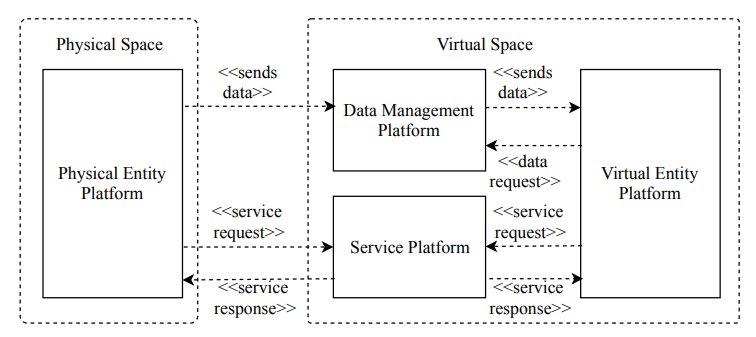
\includegraphics[width=0.7\textwidth]{Images/DT_diagram.png}
    \caption{\textbf{A Typical Digital Twin Framework}~\cite{8823809} \\
    The entities comprising the Physical Entity Platform send
specific data to the Data Management Platform. On request,
this platform sends data to the Virtual Entity Platform. The
Virtual Entity Platform can request concrete services from the
Service Platform and it receives back concrete information.
Furthermore, the underlying Physical Nodes of the Physical
Entity Platform can also send a service request to the Service
Platform and receive an appropriate response.
}
    \label{fig:DT_diagram}
\end{figure}


Simulation remains at the core of digital twin applications. Studies 
classify applications into \emph{simulation}, \emph{monitoring}, and 
\emph{control} purposes~\cite{Enders2019}. For EV charging, simulation 
provides the foundation to evaluate control strategies, optimize energy 
flows, and quantify environmental impacts. Discrete-event simulation 
platforms, such as OPTIMUS, extend these capabilities by integrating 
building energy use, grid events, and charging policies, allowing 
benchmarking of control algorithms under realistic conditions~\cite{Talusan2024}. 

In summary, digital twins bridge physical EV charging infrastructure 
with advanced simulation environments, enabling not only better 
operational decision-making but also long-term strategic planning. 
Their role as predictive, adaptive, and testable cyber-physical 
representations underscores their potential in achieving sustainable, 
resilient, and user-centric charging ecosystems.

\subsection{Data Models and Interoperability in Digital Twins}

Digital twins function as high-fidelity virtual counterparts of physical systems, supporting real-time monitoring, simulation, and control. However, realizing their full potential hinges on seamless data interoperability—the ability of multiple systems to exchange, interpret, and act upon shared information. Without standardized representations, digital twin implementations often remain siloed, each relying on proprietary formats that limit aggregation and coordinated analysis across domains~\cite{David2024}. Addressing this fragmentation requires robust standards and transformation mechanisms to align heterogeneous digital twin models, such as the Digital Twin Definition Language (DTDL) and the Asset Administration Shell (AAS)~\cite{Schmidt2023}.

Data models and ontologies play a crucial role in enabling interoperability. They provide a shared vocabulary and structure that allow systems to interpret information consistently across semantics, constraints, and behaviors~\cite{Karabulut2023}. Semantic technologies, knowledge graphs, and ontology-based integration frameworks are increasingly used to bridge modeling languages and domains, facilitating automated data fusion and richer collaboration between digital twins~\cite{Dunbar2022}. In addition, conceptual interoperability frameworks, such as those proposed by the Digital Twin Consortium, define atomic data entities and standardized messaging patterns to support modular composition of digital twins across system boundaries~\cite{Budiardjo2021}.

For infrastructures such as electric vehicle (EV) charging networks, interoperable data models are indispensable. They enable cross-system coordination between charging stations, grid services, and building energy systems; support automated integration of sensor data, user behavior, and energy flows; and provide a foundation for composable architectures where charging, storage, and renewable generation twins can interact within a unified ecosystem. Ensuring accurate, semantic-level interoperability is thus a prerequisite for building comprehensive, reliable, and scalable digital twin systems that can address the challenges of sustainable and intelligent mobility.


% \section{Inclure des images}



% \begin{figure}[ht!]
%     \centering
%     \includegraphics[width=0.35\textwidth]{example-image-a}
%     \includegraphics[width=0.35\textwidth]{example-image-b}
%     \caption{\textbf{Titre.} \lipsum[1][1-5]}
%     \label{fig:image2}
% \end{figure}



% \section{Listes et tableaux}

% \textbf{Insérer une liste~:}
% \begin{itemize}
%     \item Premier niveau
%     \begin{itemize}
%         \item[(i)] Deuxième niveau
%         \item[(ii)] Un autre élément au deuxième niveau
%     \end{itemize}
%     \item Un autre élément au premier niveau
%         \begin{itemize}
%         \item[(a)] Deuxième niveau
%         \item[(b)] Un autre élément au deuxième niveau
%     \end{itemize}
% \end{itemize}
% \bigskip

% \textbf{Insérer un tableau simple~:} 
% \begin{table}[H]
%     \centering
%     \begin{tabular}{|c|c|c|c|c|c|c|c|c|c|}
%         \hline
%         A & B & C & D & E & F & G & H & I & \dots \\
%         \hline
%         1 & 2 & 3 & 4 & 5 & 6 & 7 & 8 & 9 & \dots\\
%         10 & 11 & 12 & 13 & 14 & 15 & 16 & 17 & 18 & \dots \\
%         \hline
%     \end{tabular}
%     \caption{\textbf{Titre.} \lipsum[1][1-3]}
%     \label{tab:table-label}
% \end{table}

% \textbf{Autre style de tableau~:} 
% \begin{table}[H]
%     \centering
%     \begin{tabular}{c c c c c}
%         \hline
%         \textbf{Col1} & \textbf{Col2} & \textbf{Col3} & \textbf{Col4} & \textbf{Col5} \\
%         \hline
%         1 & 2 & 3 & 4 & 5 \\
%         1 & 2 & 3 & 4 & 5 \\
%         \hline
%     \end{tabular}
%     \caption{\textbf{Titre.} \lipsum[1][1-3]}
%     \label{tab:table-label}
% \end{table}


% \section{Insertion de code Python}
% \textbf{Insérer du code en \textit{inline}~:} \texttt{print("Hello, World!")}.\\


% \textbf{Insérer du code en \textit{inline} avec coloration syntaxique~:} \mintinline{python}{print("Hello, World!")}.\\

% \textbf{Insérer du code en bloc avec coloration syntaxique~:} 
% \begin{minted}[bgcolor=codebg,fontsize=\small,frame=lines,linenos]{python}
% def factorial(n):
%     if n == 0:
%         return 1
%     else:
%         return n * factorial(n - 1)

% # Example usage
% print(factorial(5))  # Output: 120
% \end{minted}



% \section{Expressions mathématiques}
% \subsection{Théorèmes, propositions, définitions, lemmes, demonstrations...}

% \begin{theorem}
%     \lipsum[1][1-4]
% \end{theorem}

% \begin{proof}
%     \lipsum[1][1-4]
% \end{proof}

% \begin{proposition}
%     \lipsum[1][1-4]
% \end{proposition}

% \begin{definition}
%     \lipsum[1][1-4]
% \end{definition}

% \begin{remark}
%     \lipsum[1][1-4]
% \end{remark}

% \begin{lemma}
%     \lipsum[1][1-4]
% \end{lemma}


% \subsection{Equations et calculs sur plusieurs lignes}

% \subsubsection*{Une simple équation}
% \begin{equation}
%     e = mc^2
% \end{equation}

% \subsubsection*{Une équation sur plusieurs lignes}
% \begin{equation}
%     \begin{split}
%         \mathbb{E}(aX + Y) &= \mathbb{E}(aX) + Y\\
%                            &= a\mathbb{E}(X) + Y
%     \end{split}
% \end{equation}

% \subsubsection*{Une équation avec plusieurs cas}
% \begin{equation}
%     u_n =
%     \begin{cases}
%         1 \text{ if } n\equiv0 \mod 2\\
%         0 \text{ if } n\equiv1 \mod 2 \\
%     \end{cases}
% \end{equation}

% \subsubsection*{Insérer une série de calculs}
% \begin{align*}
%     x &= 0.999\ldots \\
%     10x &= 9.999\ldots \\
%     10x - x &= 9.999\ldots - 0.999\ldots \\
%     9x &= 9 \\
%     x &= 1 \\
%     0.999\ldots &= 1
% \end{align*}

% \subsection{Utilisation du glossaire}

% \newglossaryentry{esperance}{
%     name=espérance,
%     description={Valeur moyenne théorique d'une variable aléatoire}
% }


% Référence au glossaire : \gls{esperance}.  





\chapter{Related work}\label{chap3}

\section{Brick}
Brick is a uniform metadata schema designed to represent building
entities—such as equipment, sensors, and spatial locations—and the
relationships between them using an ontology-based framework~\cite{Balaji2016Brick}.
The project was initiated by a consortium of U.S. and European
universities and research institutes, including UC Berkeley, UCLA,
Carnegie Mellon University, UC San Diego, University of Virginia,
University of Southern Denmark, and IBM Research Ireland.
The work was first presented at ACM BuildSys 2016 and continues
to evolve under the open-source Brick Schema community
(\url{https://brickschema.org}).


It addresses the interoperability challenges of heterogeneous Building
Management Systems (BMS), where vendor-specific naming and label
inconsistencies hinder the portability of applications. Brick defines a
normalized vocabulary (tags and tag sets) along with fundamental
relationships like \emph{hasPoint}, \emph{isPartOf}, \emph{feeds}, and
\emph{controls}, enabling semantic queries over RDF-based knowledge
graphs via SPARQL.

\begin{figure}[ht!]
    \centering
    
\includegraphics[width=0.7\textwidth]{Images/Basic_RDF_Graph.svg}
    \caption{\textbf{An RDF graph with triple connecting:}\\ a subject, predicate, and object}
    \label{fig:RDF}
\end{figure}

A key design choice of Brick is its reliance on the Resource
Description Framework (RDF). RDF is a W3C standard data model for
representing information as a graph of triples, each consisting of a
\emph{subject}, \emph{predicate}, and \emph{object}. For example, a
triple may state that “Room~101 \emph{hasPoint} Temperature Sensor”.
This graph-based representation allows entities and their relationships
to be linked in a uniform, machine-readable way, and queried with the
SPARQL language. By adopting RDF, Brick benefits from decades of
semantic web research, existing toolchains for reasoning, and the ability
to interoperate with other ontologies.

\begin{figure}[ht!]
    \centering
    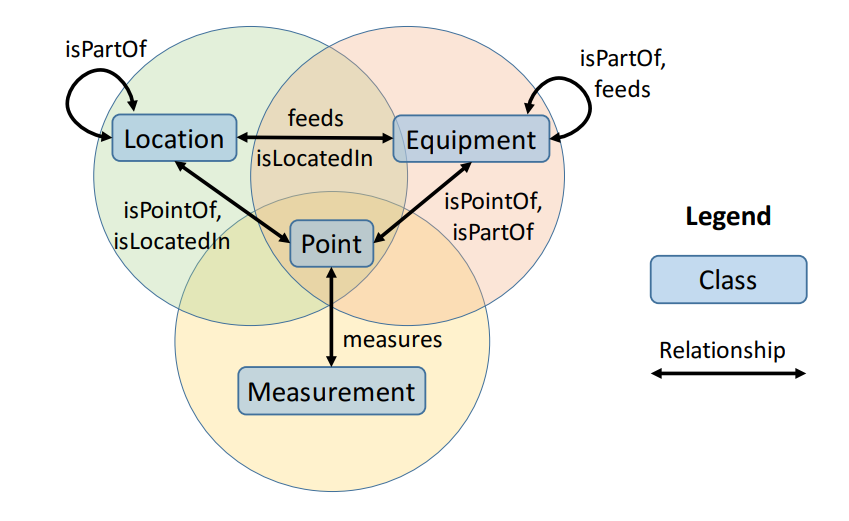
\includegraphics[width=0.7\textwidth]{Images/Brick.png}
    \caption{\textbf{Information concepts in Brick and their relationship
to a data point}~\cite{Balaji2016Brick}}
    \label{fig:Brick}
\end{figure}

Brick's key strengths include its clarity, expressiveness, and
demonstrated portability. In a validation involving six heterogeneous
buildings totaling approximately 630,000 ft\textsuperscript{2} and about
17,700 BMS data points, Brick achieved mapping coverage of around
98\% of the metadata and supported eight representative applications—
such as occupancy analytics, fault detection, demand response, and
energy apportionment—without modification~\cite{Balaji2016Brick}.
These results highlight how a compact, orthogonal schema can
significantly reduce integration costs and enable cross-site reuse of
analytics and control logic.

However, Brick also has limitations when considered in the context of
transportation systems. Its focus on static subsystems within buildings
means it lacks native constructs to represent \emph{temporal events}
(e.g., EV charging sessions), \emph{mobile entities} (e.g., vehicles), or
domain-specific regulatory and forecasting aspects. For example, a
recent evaluation of semantic technologies in building energy
flexibility found that Brick could represent only about 16\% of EV
charging–related concepts, and entirely failed to capture regulatory
constraints or environmental forecast information.
Therefore, while Brick is effective in building-scale modeling, it must
be complemented with dynamic, context-aware frameworks such as
NGSI-LD for applications in EV charging infrastructure and smart
mobility systems.

In summary, Brick combined with RDF provides a powerful and
well-structured way to model static building metadata, making
equipment, sensors, and spaces machine-readable and portable across
sites. The use of RDF triples and SPARQL enables interoperability and
semantic reasoning that are essential for digital twin applications at the
building scale. Nevertheless, Brick is less suited to domains that require
continuous handling of dynamic, time-varying data and mobile entities,
such as transportation systems and EV charging infrastructures. These
scenarios demand data models capable of representing temporal events,
context updates, and cross-domain interactions in real time. 

\section{Web of Things (WoT)}

The WoT initiative began around 2014 within the World Wide Web Consortium (W3C) Interest Group
and was formalized in the WoT Working Group, with the first
recommendations—covering the WoT Architecture and the Thing
Description—published in 2020~\cite{W3CWOT2020}.W3C is an international standards
organization founded in the United States in 1994 but with a
globally distributed membership and governance.

At its core is the \emph{Thing Description} (TD), a machine-readable
document based on JSON-LD that specifies the metadata, properties,
actions, and events of a device~\cite{W3CWOT2020}. A TD serves as a
semantic contract between a device (the “Thing”) and applications,
allowing developers to interact with devices through uniform APIs
regardless of vendor-specific protocols.

\begin{figure}[ht]
    \centering
    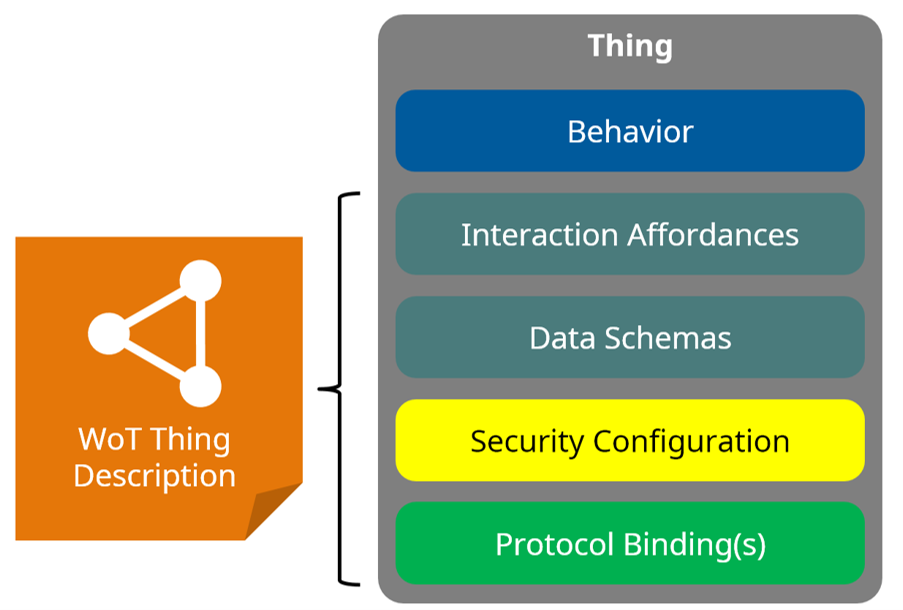
\includegraphics[width=0.3\textwidth]{Images/td.png}
    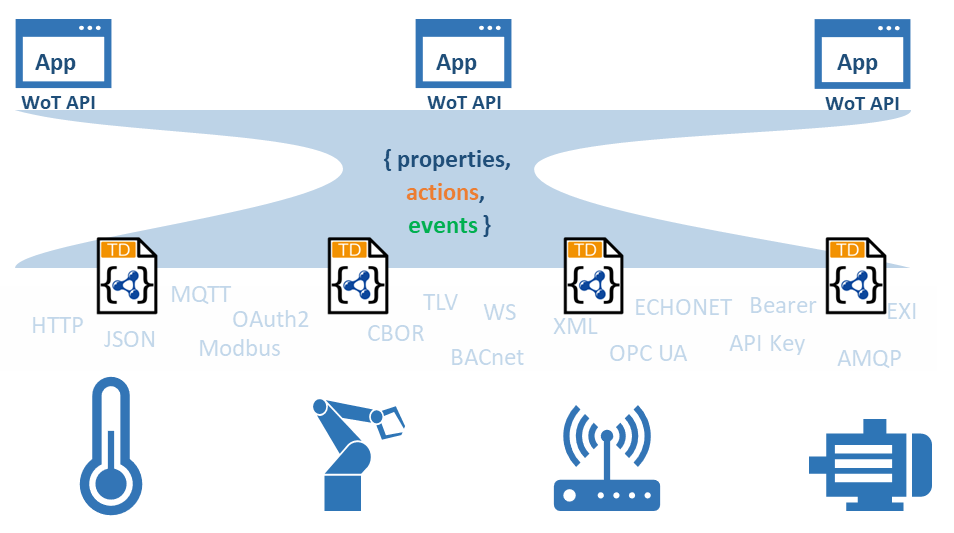
\includegraphics[width=0.35\textwidth]{Images/wot-mappings.png}
    \caption{\textbf{IoT Metadata in TD (left) and WoT mappings (right)} \\In general, WoT is a protocol agnostic approach and provides a common mechanism to define how specific protocols such as MQTT, HTTP, CoAP or Modbus can be mapped to the WoT's interaction properties-action-event abstraction.~\cite{W3CWOT2020}}
    \label{fig:image2}
\end{figure}


The strengths of WoT lie in its ability to provide a lightweight,
technology-agnostic abstraction for devices. By describing
functionalities in JSON-LD, WoT enables semantic interoperability
between devices that expose different protocols (e.g., HTTP, CoAP,
MQTT). This abstraction facilitates integration of IoT devices into
larger ecosystems, allowing web applications, gateways, and digital
twin platforms to discover and use device capabilities in a consistent
way. The WoT standard is also modular, supporting security,
binding templates, and scripting APIs, which together ease the
deployment of scalable IoT systems.

Despite these advantages, WoT also has limitations when applied to
transportation and EV charging infrastructure. WoT focuses on the
device level—standardizing access to sensors and actuators—but it
does not by itself provide higher-level semantics for systems such as
charging networks, mobility services, or energy markets. As a result,
WoT alone cannot capture domain-specific relationships (e.g., vehicle
arrival events linked to charging tariffs, or the coordination between
multiple charging stations). In practice, WoT is most effective when
used in combination with higher-level frameworks which can
forming a layered approach to interoperability in smart transport
systems.

\section{FIWARE and NGSI-LD}

FIWARE is an open-source platform initiative launched in 2011 under
the European Union’s Seventh Framework Programme (FP7), initially
supported by the European Commission and a consortium of European
companies and research organizations. It is now managed by the
FIWARE Foundation, a non-profit association based in Berlin, Germany,
which coordinates global adoption of FIWARE technologies across smart
cities, energy, industry, and mobility. At the heart of FIWARE is the
\emph{Context Broker}, the core component that manages context
information about entities in the physical and digital world. The most
widely used implementation is the Orion Context Broker and its
NGSI-LD compliant extension Orion-LD.

\begin{figure}[ht]
    \centering
    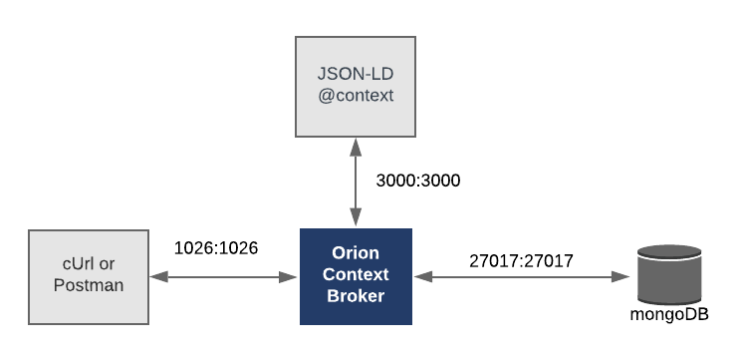
\includegraphics[width=0.7\textwidth]{Images/orion.png}
    \caption{\textbf{Orion Context Broker Architecture}}
    \label{fig:orion}
\end{figure}

The FIWARE Next Generation Service Interfaces (NGSI) define the
standard API for context management. NGSI-LD, standardized by ETSI
(European Telecommunications Standards Institute) in 2019, extends
earlier NGSI versions by adopting linked-data principles and JSON-LD
serialization~\cite{ETSI2019NGSILD}. It provides an entity–property–
relationship model that is semantically interoperable and aligned with
semantic web technologies. Each NGSI-LD entity can represent a
real-world object (e.g., an EV charging station), its properties (e.g.,
capacity, current load), and its relationships (e.g., connected to a power
grid or located in a district). The Context Broker exposes these entities
via a publish–subscribe API, allowing real-time updates and
notifications.

The strengths of FIWARE and NGSI-LD lie in their ability to handle
\emph{dynamic context} at scale. Through the Context Broker,
applications can subscribe to changes (e.g., a vehicle starting or
ending a charging session) and react immediately. This dynamic and
event-driven model is particularly advantageous in domains such as
transport and energy, where continuous synchronization with rapidly
changing environments is required. FIWARE also provides a broad
ecosystem of enablers—such as IoT agents, data processing
components, and dashboards—that simplify integration with IoT
devices and data platforms, facilitating large-scale deployments in
smart cities worldwide~\cite{Papadakis2022NGSI}.

Nevertheless, FIWARE and NGSI-LD also present challenges when
applied to transportation and EV charging infrastructure. While
NGSI-LD defines a generic model, it does not provide detailed domain
semantics for vehicles, tariffs, or multimodal transport flows. Developers
often rely on the \emph{Smart Data Models} initiative, jointly maintained
by the FIWARE Foundation, ETSI, and the Open \& Agile Smart Cities
(OASC) network, to obtain domain-specific schemas. Furthermore,
heterogeneous modeling practices across projects can hinder semantic
consistency, and complex cross-domain interactions (e.g., integrating
mobility services with energy markets) often require additional semantic
integration layers. 

\section{Internship Challenges and Contribution}

The analysis of related frameworks highlights that Brick, WoT, and
FIWARE/NGSI-LD each address different layers of interoperability.
Brick provides a static ontology for building metadata, WoT enables
device-level interoperability via standard Web interfaces, and
FIWARE/NGSI-LD offers a scalable framework for dynamic context
management in smart environments. Table~\ref{tab:comparison}
summarizes their origins, strengths, and limitations.

\begin{table}[htb]
\centering
\caption{Comparison of FIWARE, Brick, and WoT}
\label{tab:comparison}
\renewcommand{\arraystretch}{1.3} % 增加行间距
\begin{tabular}{|>{\raggedright\arraybackslash}p{2.8cm}|>{\raggedright\arraybackslash}p{4cm}|>{\raggedright\arraybackslash}p{4cm}|>{\raggedright\arraybackslash}p{4cm}|}
\hline
\textbf{Aspect} & \textbf{FIWARE} & \textbf{Brick} & \textbf{WoT} \\ 
\hline\hline
\textbf{Main focus} & 
Dynamic context management through Context Broker and NGSI-LD API & 
Semantic ontology framework for building metadata and relationships & 
Device interoperability via Web standards and protocols \\ 
\hline
\textbf{Modeling method} & 
NGSI-LD (Linked Data with JSON-LD serialization) & 
RDF + OWL ontology with SPARQL queries & 
Thing Description using JSON-LD and Web APIs \\ 
\hline
\textbf{Pros} & 
\begin{itemize}[leftmargin=*,nosep,after=\strut]
\item Real-time context updates
\item Subscription mechanisms
\item Cross-domain interoperability
\item Scalable REST APIs
\end{itemize} & 
\begin{itemize}[leftmargin=*,nosep,after=\strut]
\item Unified building semantics
\item Strong reasoning capabilities
\item Rich relationship modeling
\item Standardized vocabulary
\end{itemize} & 
\begin{itemize}[leftmargin=*,nosep,after=\strut]
\item Protocol-agnostic access
\item Standardized APIs
\item Web integration
\item Device abstraction
\end{itemize} \\ 
\hline
\textbf{Cons} & 
\begin{itemize}[leftmargin=*,nosep,after=\strut]
\item Limited domain ontologies
\item Depends on Smart Data Models
\item Device-level control constraints
\end{itemize} & 
\begin{itemize}[leftmargin=*,nosep,after=\strut]
\item Weak dynamic data handling
\item Limited temporal modeling
\item Mainly static metadata focus
\end{itemize} & 
\begin{itemize}[leftmargin=*,nosep,after=\strut]
\item Weak semantic reasoning
\item Limited complex system modeling
\item Primarily device-layer focus
\end{itemize} \\ 
\hline
\textbf{Organization} & 
FIWARE Foundation and ETSI & 
Brick Schema community & 
W3C \\ 
\hline
\end{tabular}
\end{table}

From this comparison, it becomes evident that while Brick and WoT
provide valuable capabilities, they are not sufficient for the specific
challenges of modeling and managing electric vehicle (EV) charging
infrastructure. Brick is too static to capture real-time charging events,
and WoT does not extend beyond device-level descriptions. In
contrast, FIWARE and its NGSI-LD standard are designed for
real-time, cross-domain interoperability and have already been
adopted in numerous European smart city and energy projects.

Given that this research is funded within the European context, FIWARE/NGSI-LD is a natural choice as it is an EU
initiative, standardized by ETSI, and actively supported by the FIWARE
Foundation. Beyond alignment with funding priorities, FIWARE is also
technically best suited for the EV charging scenario, as it provides the
necessary dynamic context management, integration of IoT data, and
publish–subscribe mechanisms required for real-time infrastructure
simulation.

\textbf{Challenges.} Despite these advantages, several research
challenges must be addressed:
\begin{itemize}
  \item \emph{Heterogeneous data sources:} EV charging systems involve
  multiple actors (vehicles, stations, grid, users) that produce data in
  diverse formats, requiring semantic harmonization.
  \item \emph{Dynamic context management:} Unlike static building
  systems, charging infrastructure generates highly dynamic data such
  as charging sessions, user arrivals, and fluctuating grid loads, which
  must be represented in real time.
  \item \emph{Cross-domain interoperability:} Integration across energy,
  mobility, and urban systems demands models that can capture
  relationships beyond the device or building level.
  \item \emph{Scalability and performance:} Digital twins for large-scale
  charging networks must support efficient storage, querying, and
  notification mechanisms under high data volume.
\end{itemize}

\textbf{Contributions.} Building on this motivation, the main
contributions of this work are as follows:
\begin{itemize}
  \item Design and implementation of a digital twin framework for EV
  charging infrastructure based on FIWARE and NGSI-LD.
  \item Development of NGSI-LD compliant data models that capture
  both charging station characteristics and user behavior in dynamic
  contexts.
  \item Integration of databases and APIs for real-time monitoring,
  simulation, and analysis of charging infrastructure performance.
  \item Demonstration of how the proposed platform can support
  deployment strategies, demand forecasting, and optimization of EV
  charging networks.
\end{itemize}





% \section{Listes et tableaux}

% \textbf{Insérer une liste~:}
% \begin{itemize}
%     \item Premier niveau
%     \begin{itemize}
%         \item[(i)] Deuxième niveau
%         \item[(ii)] Un autre élément au deuxième niveau
%     \end{itemize}
%     \item Un autre élément au premier niveau
%         \begin{itemize}
%         \item[(a)] Deuxième niveau
%         \item[(b)] Un autre élément au deuxième niveau
%     \end{itemize}
% \end{itemize}
% \bigskip

% \textbf{Insérer un tableau simple~:} 
% \begin{table}[H]
%     \centering
%     \begin{tabular}{|c|c|c|c|c|c|c|c|c|c|}
%         \hline
%         A & B & C & D & E & F & G & H & I & \dots \\
%         \hline
%         1 & 2 & 3 & 4 & 5 & 6 & 7 & 8 & 9 & \dots\\
%         10 & 11 & 12 & 13 & 14 & 15 & 16 & 17 & 18 & \dots \\
%         \hline
%     \end{tabular}
%     \caption{\textbf{Titre.} \lipsum[1][1-3]}
%     \label{tab:table-label}
% \end{table}

% \textbf{Autre style de tableau~:} 
% \begin{table}[H]
%     \centering
%     \begin{tabular}{c c c c c}
%         \hline
%         \textbf{Col1} & \textbf{Col2} & \textbf{Col3} & \textbf{Col4} & \textbf{Col5} \\
%         \hline
%         1 & 2 & 3 & 4 & 5 \\
%         1 & 2 & 3 & 4 & 5 \\
%         \hline
%     \end{tabular}
%     \caption{\textbf{Titre.} \lipsum[1][1-3]}
%     \label{tab:table-label}
% \end{table}


% \section{Insertion de code Python}
% \textbf{Insérer du code en \textit{inline}~:} \texttt{print("Hello, World!")}.\\


% \textbf{Insérer du code en \textit{inline} avec coloration syntaxique~:} \mintinline{python}{print("Hello, World!")}.\\

% \textbf{Insérer du code en bloc avec coloration syntaxique~:} 
% \begin{minted}[bgcolor=codebg,fontsize=\small,frame=lines,linenos]{python}
% def factorial(n):
%     if n == 0:
%         return 1
%     else:
%         return n * factorial(n - 1)

% # Example usage
% print(factorial(5))  # Output: 120
% \end{minted}



% \section{Expressions mathématiques}
% \subsection{Théorèmes, propositions, définitions, lemmes, demonstrations...}

% \begin{theorem}
%     \lipsum[1][1-4]
% \end{theorem}

% \begin{proof}
%     \lipsum[1][1-4]
% \end{proof}

% \begin{proposition}
%     \lipsum[1][1-4]
% \end{proposition}

% \begin{definition}
%     \lipsum[1][1-4]
% \end{definition}

% \begin{remark}
%     \lipsum[1][1-4]
% \end{remark}

% \begin{lemma}
%     \lipsum[1][1-4]
% \end{lemma}


% \subsection{Equations et calculs sur plusieurs lignes}

% \subsubsection*{Une simple équation}
% \begin{equation}
%     e = mc^2
% \end{equation}

% \subsubsection*{Une équation sur plusieurs lignes}
% \begin{equation}
%     \begin{split}
%         \mathbb{E}(aX + Y) &= \mathbb{E}(aX) + Y\\
%                            &= a\mathbb{E}(X) + Y
%     \end{split}
% \end{equation}

% \subsubsection*{Une équation avec plusieurs cas}
% \begin{equation}
%     u_n =
%     \begin{cases}
%         1 \text{ if } n\equiv0 \mod 2\\
%         0 \text{ if } n\equiv1 \mod 2 \\
%     \end{cases}
% \end{equation}

% \subsubsection*{Insérer une série de calculs}
% \begin{align*}
%     x &= 0.999\ldots \\
%     10x &= 9.999\ldots \\
%     10x - x &= 9.999\ldots - 0.999\ldots \\
%     9x &= 9 \\
%     x &= 1 \\
%     0.999\ldots &= 1
% \end{align*}

% \subsection{Utilisation du glossaire}

% \newglossaryentry{esperance}{
%     name=espérance,
%     description={Valeur moyenne théorique d'une variable aléatoire}
% }


% Référence au glossaire : \gls{esperance}.  






%%% Glossaire %%%
\printglossaries


%%% Appendix %%%
\appendix

\chapter{Annexe}
\subsection*{\Large Annexe 1 - List of Interviewees (Chapter 6)}

\begin{itemize}
    \item \textbf{Dr.Daphne Tuncer:} Chercheure ENPC
    \item \textbf{Dr.Georgios Bouloukakis:} Assistant Professor at University of Patras
\end{itemize}


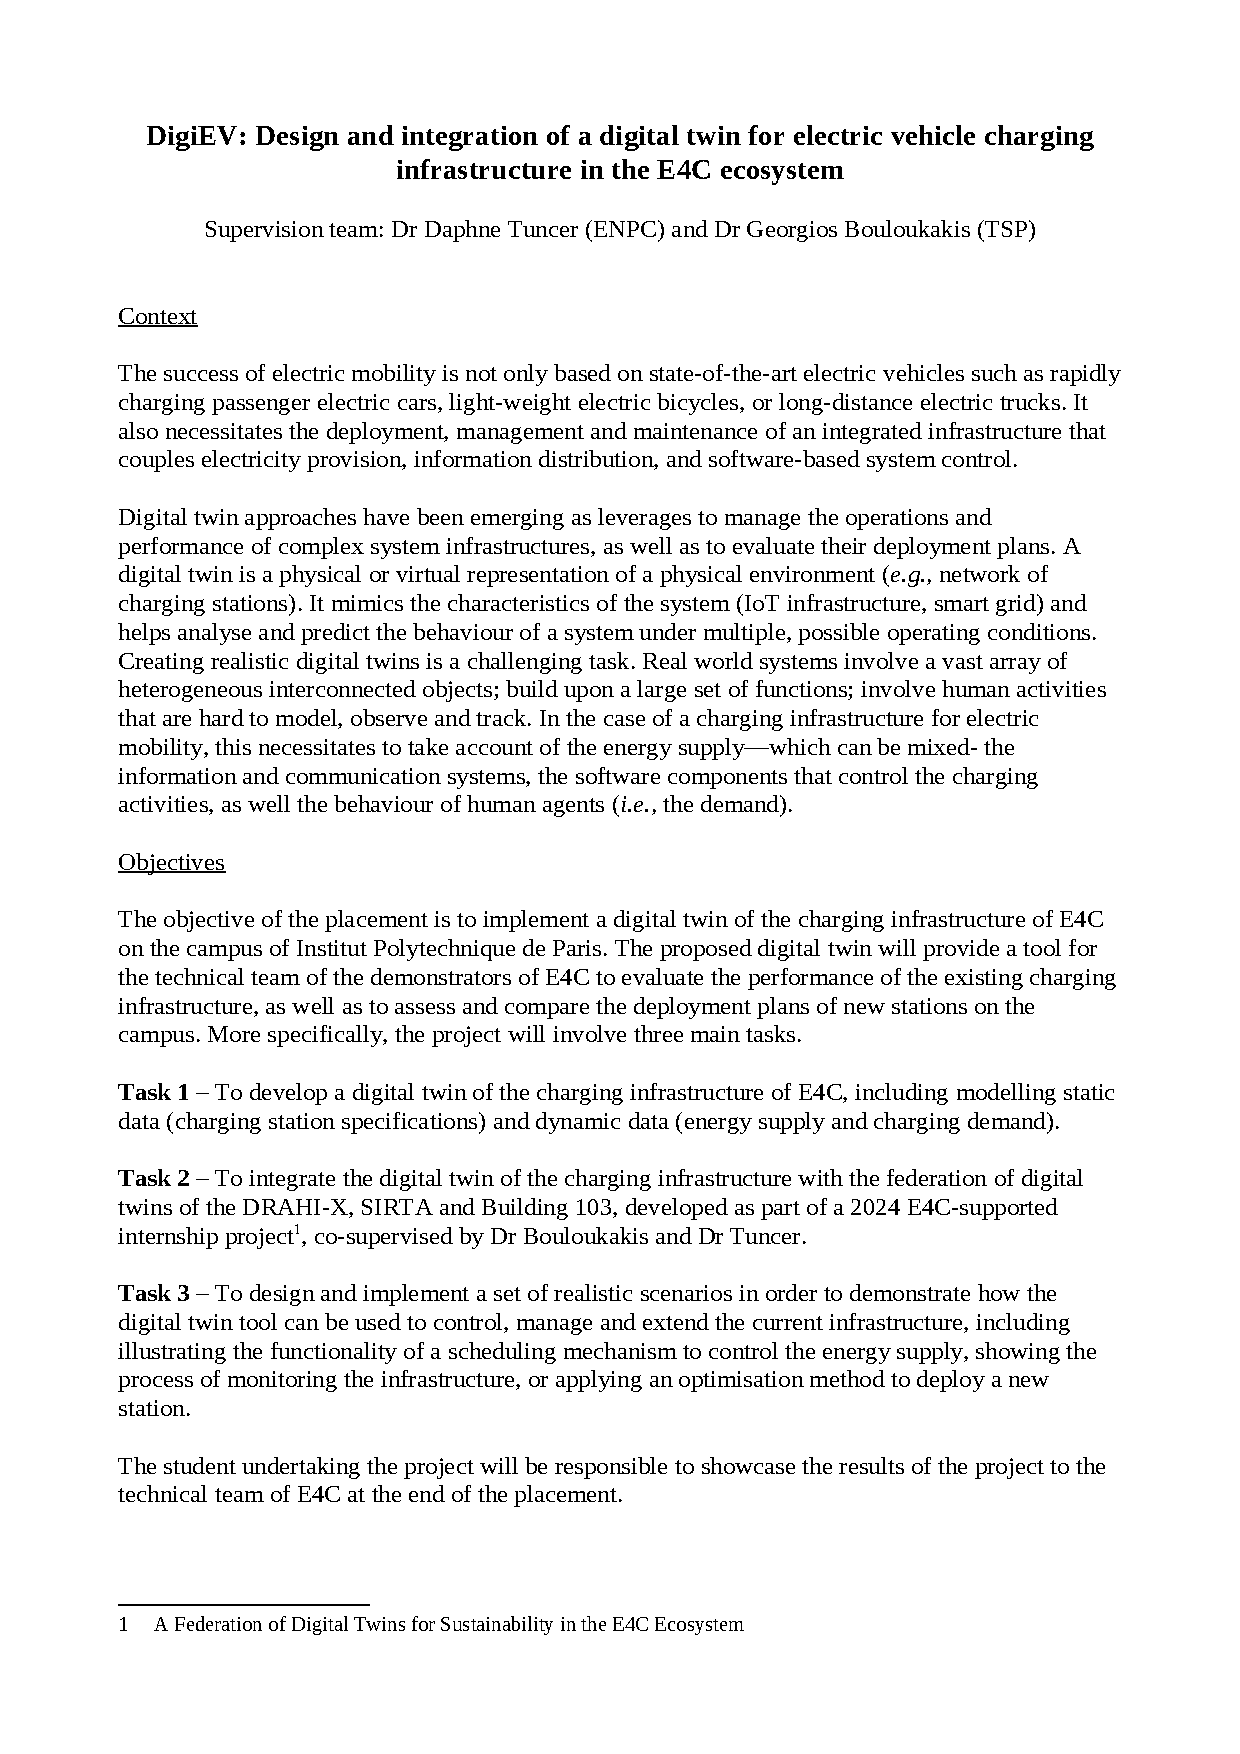
\includepdf[pages=1,scale=0.8,pagecommand={
    \begin{minipage}{\textwidth}
    \centering
    \vspace{0cm}
    {\Large \textbf{Annexe 2 - Internship Advertisement}}
    \raggedright
    \end{minipage}
}]{Images/electricMobilityDigitalTwin_projectDescription_2025.pdf}
\includepdf[pages=2-,scale=0.8]{Images/electricMobilityDigitalTwin_projectDescription_2025.pdf}


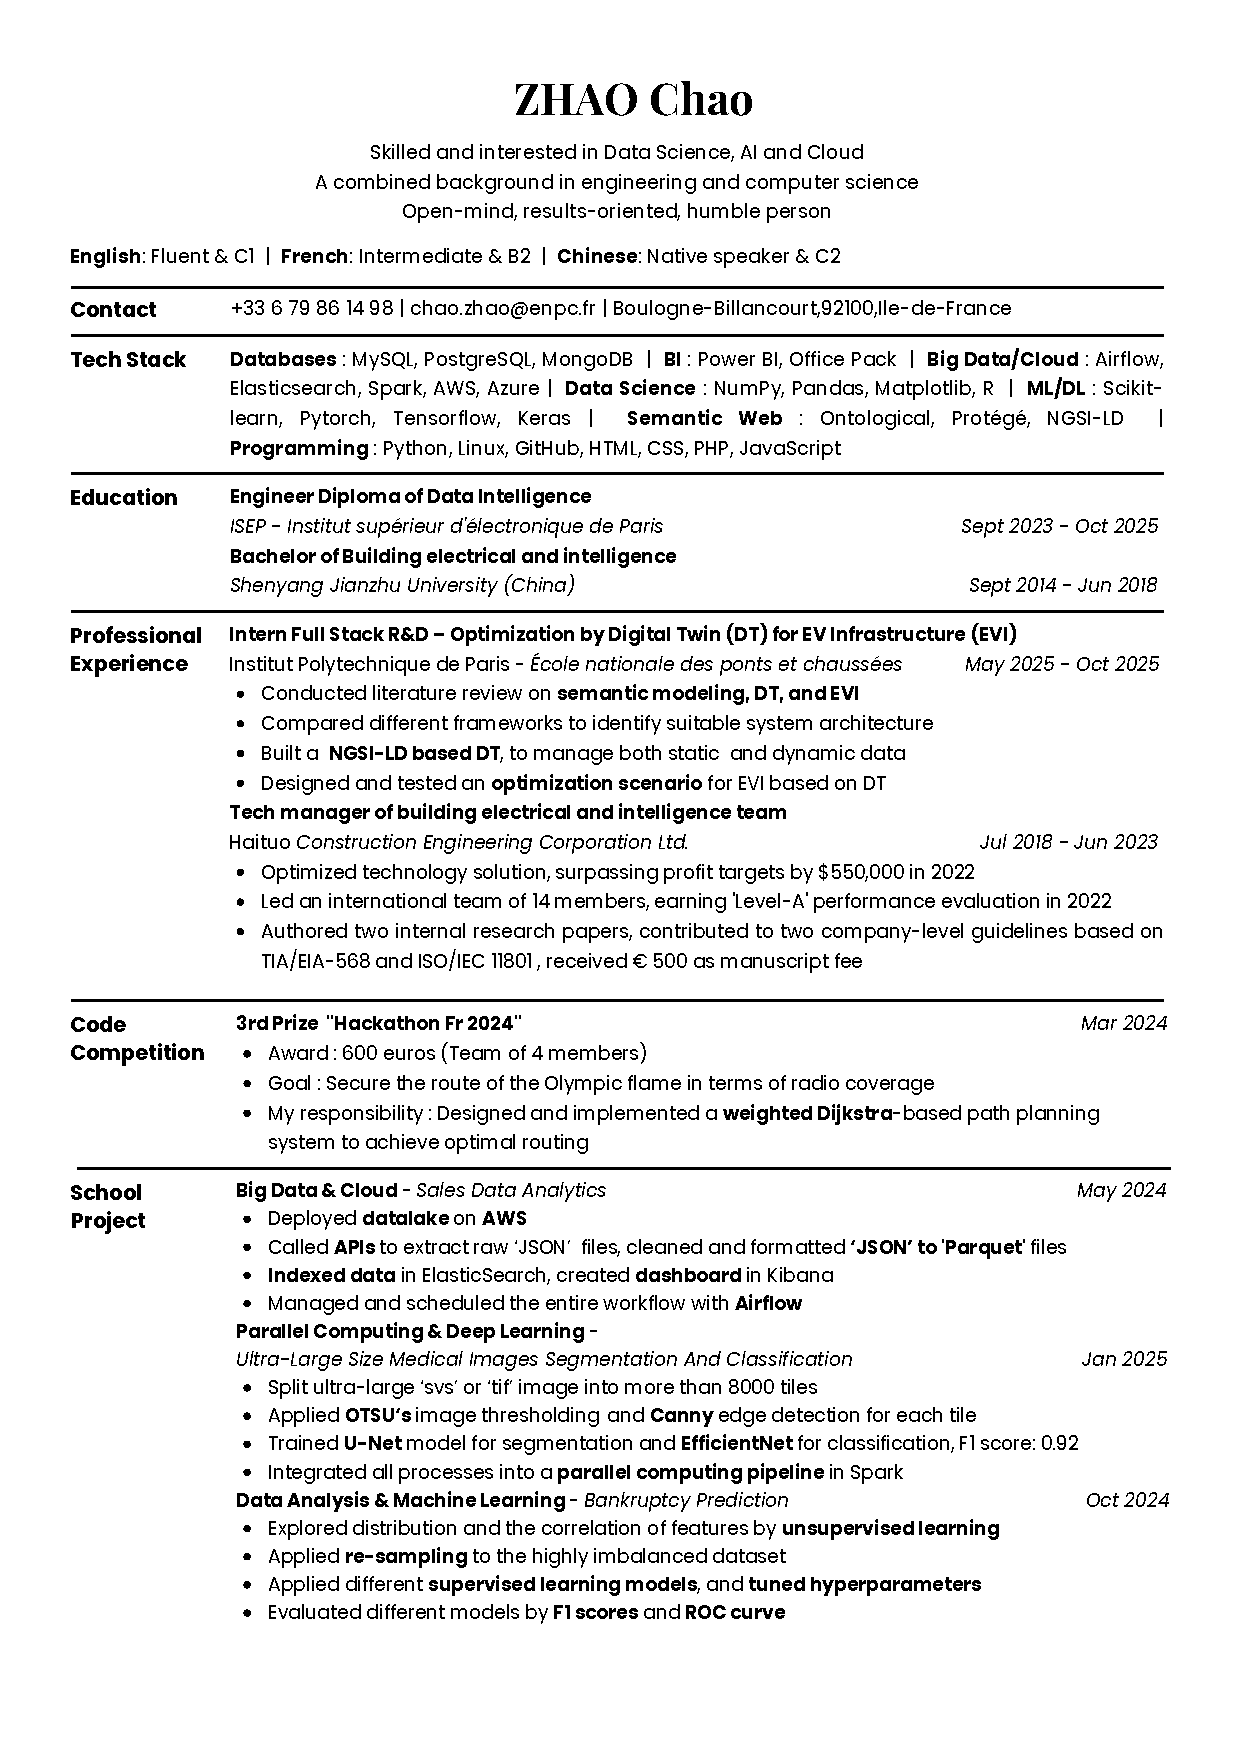
\includepdf[pages=1,scale=0.8,pagecommand={
    \begin{minipage}{\textwidth}
    \centering
    \vspace{0cm}
    {\Large \textbf{Annexe 3 - CV}}
    \raggedright
    \end{minipage}
    }]{Images/cv.pdf}
    \newpage


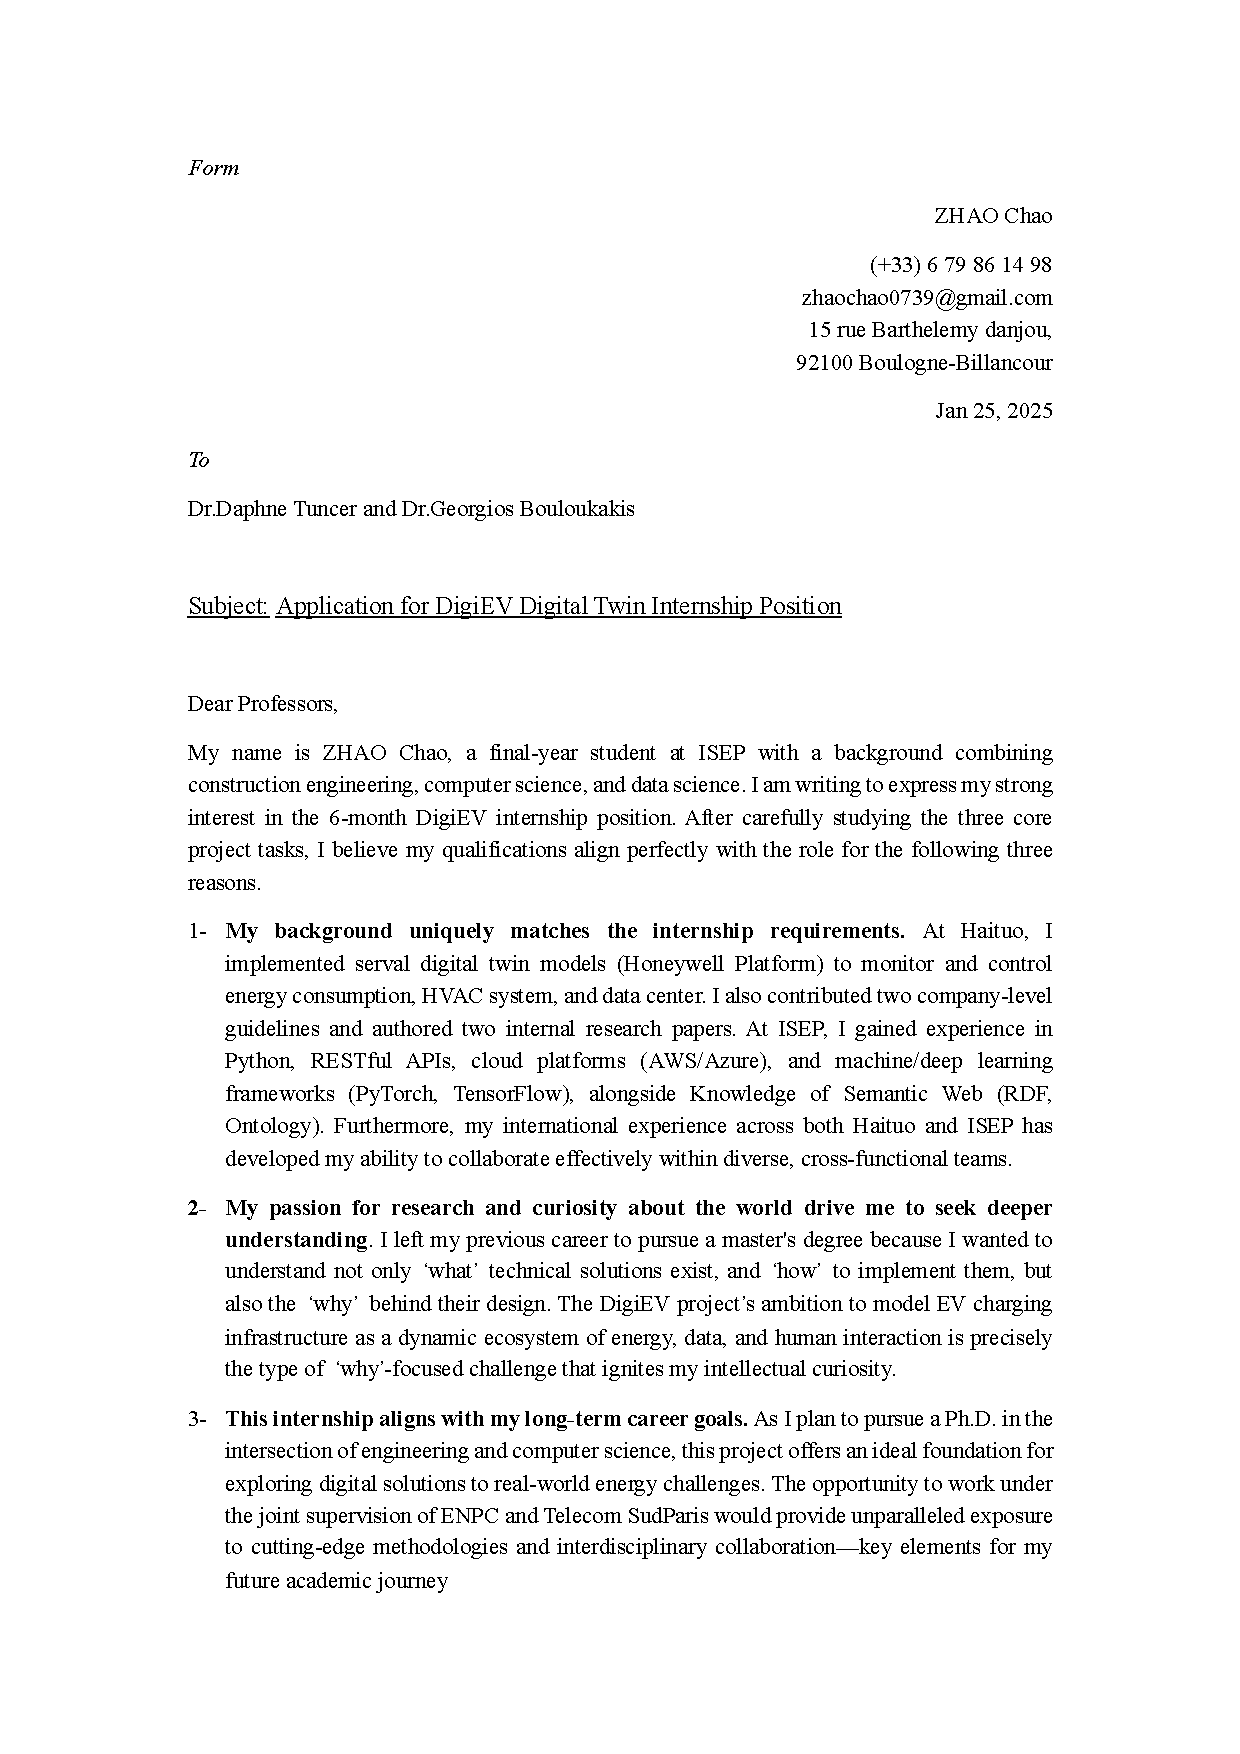
\includepdf[pages=1,scale=0.8,pagecommand={
    \begin{minipage}{\textwidth}
    \centering
    \vspace{0cm}
    {\Large \textbf{Annexe 4 - Motivation Letter}}
    \raggedright
    \end{minipage}
}]{Images/Motivation Letter.pdf}
\includepdf[pages=2-,scale=0.8]{Images/Motivation Letter.pdf}




\urlstyle{same}


%%% Bibliography %%%
\bibliographystyle{unsrt} 
\bibliography{References}

\end{document}

